\chapter{Astrophysical Messengers}\label{chapter:astromessengers}
This work will focus primarily on cosmic rays, photons, and neutrinos, however other messengers, such as gravitational waves, can provide unique information as well. 

\section{Cosmic Rays}
\subsection{Energy Spectrum}
Cosmic rays are high energy protons and atomic nuclei, originating from outside the Earth's atmosphere. It is difficult to do traditional astronomy  using cosmic rays (in the sense of using their arrival directions to identify sources) due to the fact that cosmic rays are charged, and consequently their paths are bent by magnetic fields in the universe. However, the cosmic ray spectrum is well studied, with many measurements having been made over the past century since their initial discovery. In general, the spectrum can be modeled as a power law (eq.~\ref{CRSpectEq}):

\begin{equation}
    N(E)dE \propto E^{-x}dE
\label{CRSpectEq}
\end{equation}

where N describes the number of cosmic ray particles, E is their energy, and x is an energy-dependent spectral index. The spectrum has several notable features, shown in figure~\ref{fig:CRSpectrum}. At lower energies (below $10^16$ eV), the spectrum is well described by an $E^{-2.7}$ flux. At $10^16$ eV, the spectrum softens to $E^{-3.1}$, commonly referred to as the "knee". At even higher energies (around $10^18.5$ eV), the spectrum hardens again. This region is referred to as the "ankle", and is thought to correspond to the point where extragalactic cosmic rays begin to dominate the flux. 

\begin{figure}[h]
\centering
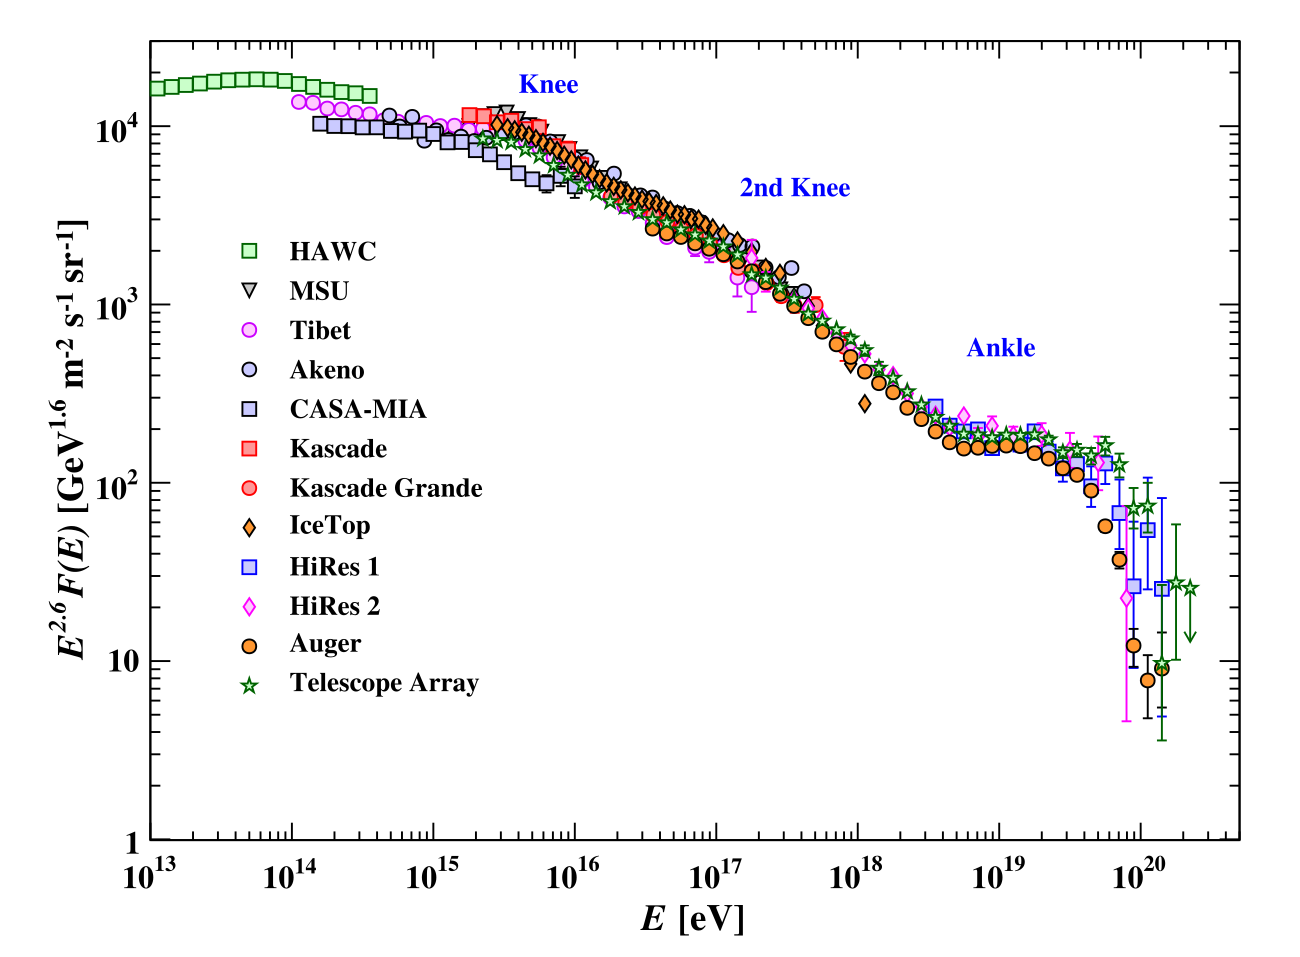
\includegraphics[width=0.8\textwidth]{figs/CR_Spectrum.png}
\caption{A plot of the cosmic ray spectrum assembled from observations from a variety of experiments. Major features visible are the knee ($\approx 10^{16} $ eV), and the ankle ($\approx 10^{19}$ eV). ~\cite{AustinThesis} }
\label{fig:CRSpectrum}
\end{figure}

\subsection{Acceleration Mechanism}
Though the exact origin of cosmic rays is still unknown, we can infer how these particles are being accelerated based on our knowledge of how charged particles behave. 
\begin{figure}[h]
\centering
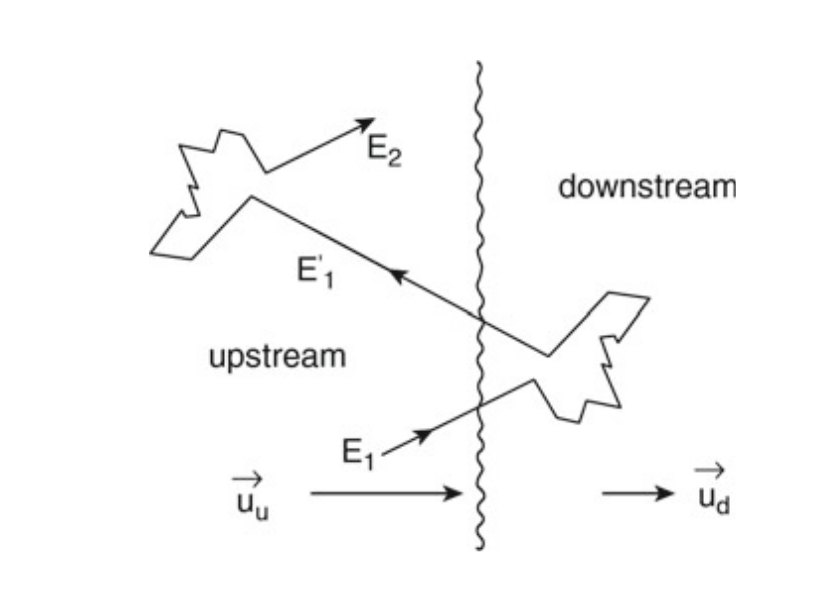
\includegraphics[width=0.8\textwidth]{figs/FermiFig.png}
\caption{Fermi acceleration of a plane shock front\cite{pimenta_partphys}. }
\label{fig:fermifig}
\end{figure}

Suppose a particle encounters a moving cloud of plasma. If it is large enough, the cloud will act as a massive scatterer. The overal collision is the result of a large number of individual scatterings inside the cloud, and the outgoing angle of the original particle is essentially random. On average the energy of the particle after a collision with this boundary will increase by a factor (eq.~\ref{secondfermieq}):

\begin{equation}
    \langle\frac{\Delta E}{E}\rangle \approx \frac{4}{3}\beta^2
\label{secondfermieq}
\end{equation}

Where $\beta=V/c$, corresponding to the boundary velocity. This is \textit{second order Fermi acceleration}, and is generally insufficient to explain the cosmic ray spectrum. If we instead assume a plane shock front, as in figure \ref{fig:fermifig} , then the post-collision velocity of the particle is no longer randomly distributed, and we instead obtain the expression (eq.~\ref{firstfermieq}):

\begin{equation}
    \langle\frac{\Delta E}{E}\rangle \approx \frac{4}{3}\beta
\label{firstfermieq}
\end{equation}

This describes \textit{first order Fermi acceleration}. From here, we can calculate the expected flux measured at Earth to be (eq.~\ref{fermiexpflux}):

\begin{equation}
    \frac{dN}{dE} \propto (\frac{E}{E_0})^{-\Gamma}
\label{fermiexpflux}
\end{equation}

where $\Gamma=\alpha+1$, $\alpha\approx \frac{3P_e}{4 \beta}$, and $P_e$ is the probability that a particle may escape the shock region (proportional to the velocity, $V$). Note that this is a power law with almost constant spectral index, as both $\beta$ and $P_e$ are proportional to $V$, similar to what is seen in the observed cosmic ray spectrum~\cite{pimenta_partphys}. 

We can additionally derive constraints on the maximum energy to which a particle can be accelerated based off the magnetic field intensity, $B$, and the size of the accelerating region, $R$ (eq.~\ref{HillasCond}):

\begin{equation}
    E_{max} = eBR \approx 10^{21} [\frac{R}{\textrm{1 pc}}][\frac{B}{\textrm{1 Gauss}}] \textrm{ eV}
\label{HillasCond}
\end{equation}

This is known as \textit{Hillas' condition}, and can inform us about the properties of cosmic ray accelerators. We can plot this condition to show sources which satisfy this requirement for a particular energy, producing what is commonly referred to as Hillas' plot (Figure \ref{fig:hillasplot}). Sources must exist above the diagonal thresholds in order to be valid accelerators of cosmic rays of certain energies. For example, sources capable of accelerating protons to ~100 EeV energies must exist above the dashed line in figure~\ref{fig:hillasplot}. Sources below are either too small, or have magenetic fields that are too weak.    

\begin{figure}[h]
\centering
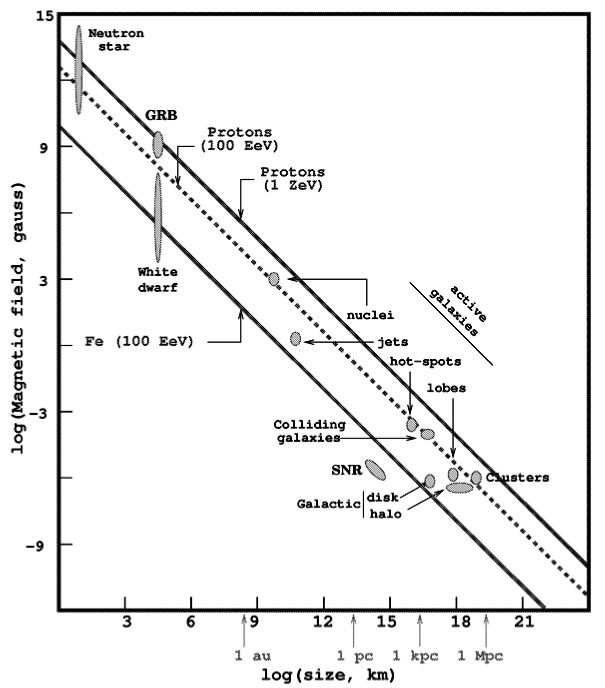
\includegraphics[width=0.8\textwidth]{figs/HillasPlot.jpg}
\caption{A Hillas plot, showing source populations capable of accelerating cosmic rays to a given energy, given their size and magnetic field strength~\cite{hillasplotsrc}.}
\label{fig:hillasplot}
\end{figure}


\section{Photons}
Perhaps the oldest and most well-studied astrophysical messenger, photons have the useful property of being electrically neutral. Unlike cosmic rays, their paths are not bent by magnetic fields, and the arrival directions of photons can be used to identify their origin, particularly at high energies due to their good angular resolution. Photons additionally span a large energy range, and can be used to explore a wide variety of astrophysical production processes. For the purposes of this work, we are most interested in the highest energy photons (gamma rays, with energies greater than 100 keV), which can be produced through either leptonic or hadronic processes.

\subsection{Leptonic Radiative Processes}
While photons cannot be directly accelerated by electric and magnetic fields, there are a variety of mechanisms by which processes involving leptons can produce high energy photons. 

\begin{itemize}
    \item \textbf{Synchrotron radiation:} Radially accelerated relativistic particles will release synchrotron radiation. This typically occurs as charged particles (such as electrons) spiral through magnetic fields. The power loss, ($dE/dT)$, due to synchrotron radiation for a particle of mass M and charge Z can be expressed as (eq. \ref{syncheq}):
    \begin{equation}
        -\frac{dE}{dT} \approx 2.6 (\frac{Zm_e}{M})^4(\frac{E}{\textrm{1 keV}})^2(\frac{B}{1\textrm{ G}})^2 \textrm{ keV s}^{-1}
    \label{syncheq}
    \end{equation}
    Where $m_e$ is the electron mass, $E$ is the particle energy, and $B$ is the magnetic field strength. From equation~\ref{syncheq} it can be seen that synchrotron emission is significantly more relevant for electrons than protons, due to the $1/M^4$ term.
    
    \item \textbf{Compton Scattering and Inverse Compton Scattering:} Photons may scatter off an electron at rest, and in doing so experience a wavelength shift according to (\ref{compeq}):
    \begin{equation}
        \frac{\lambda'-\lambda}{\lambda}=\frac{\hbar\omega}{m_e c^2}(1 - \cos\alpha)
    \label{compeq}
    \end{equation}
    Where $\lambda'$ and $\lambda$ correspond to the final and initial photon wavelengths, and $\alpha$ is the deflection angle of the photon. If a low energy photon collides with a high energy electron, the energy of the photon may exit with more energy than it began with, providing an effective mechanism for increasing the photon energy. 
\end{itemize}

A combination of these two processes can produce the two peak structure typically seen in the spectrum of observed gamma ray sources. The lower energy peak is due to synchrotron radiation, while the higher energy peak corresponds to low energy photons being scattered to higher energies via inverse compton scattering. 
    
\begin{figure}[h]
\centering
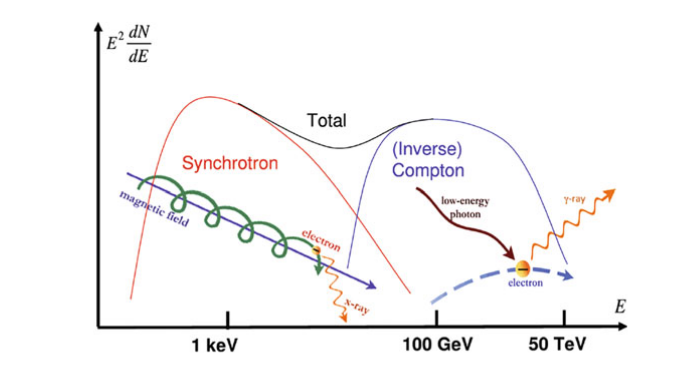
\includegraphics[width=0.8\textwidth]{figs/toygammaspect.png}
\caption{A cartoon plot of the gamma ray spectrum for a high energy gamma ray source. The two peak structure arises from the two production mechanisms of gamma rays. At lower energies, photons are produced by synchrotron radiation of electrons spiraling around magnetic field lines. The higher energy peak is then formed by the lower energy photons being scattered off energetic electrons via inverse compton scattering~\cite{pimenta_partphys_compton}. }
\label{fig:fermifig}
\end{figure}

\subsection{Hadronic Radiative Processes}
While leptonic processes can produce high energy gamma rays, hadronic processes will produce gamma rays in addition to neutrinos and cosmic rays. Protons accelerated to high energies in an astrophysical source may interact with other protons via (eq. \ref{hadeq}):

\begin{equation}
    p + p \rightarrow [\pi^0 + \pi^+ + \pi^-] + X
\label{hadeq}    
\end{equation}

Where X is the appropriate nucleus or hadron depending on the pions produced, and on average there is expected to be equal production of neutral and charged pions. Additionally, protons may interact with photons, providing an additional path to pion production (eq. \ref{hadeq2} and \ref{hadeq3}):

\begin{equation}
    p + \gamma \rightarrow \Delta^+ \rightarrow \pi^0 + p
\label{hadeq2}    
\end{equation}
\begin{equation}
    p + \gamma \rightarrow \Delta^+ \rightarrow \pi^+ + n
\label{hadeq3}    
\end{equation}

These resultant pions can subsequently decay, producing child particles depending on the particular pion type. Neutral pions will decay into gamma rays ($\pi^0 \rightarrow \gamma + \gamma$), and charged pions will decay to a lepton and their associated (anti)neutrino (most often muons and muon neutrinos: $\pi^+ \rightarrow \nu_{\mu} + \mu^+$, $\pi^- \rightarrow \bar{\nu_{\mu}} + \mu^-$). As such the sources of cosmic rays are expected to additionally produce a high energy gamma ray flux.

\subsection{Gamma Rays as an Astrophysical Messenger}
Gamma rays are a robust astrophysical messenger. As previously mentioned, photons are uncharged and their arrival directions can consequently be used to identify their origin. Additionally, the gamma ray energy can be used to infer information about the primary particle energy for a known production mechanism. Gamma rays are also well studied, and modern detectors boast high event rates: Fermi-LAT, for example, observes enough events to be capable of studying the temporal variability of sources on the timescale of approximately a day. 

Gamma rays are not without their limitations, however. Note that while at the highest energies gamma rays may be produced by both leptonic and hadronic processes, only hadronic processes are expected to additionally produce neutrinos and cosmic rays. For this reason, high energy gamma rays alone cannot be used to identify the source of high energy cosmic rays. 

Additionally, high energy gamma rays may also interact electromagnetically with the ambient radiation in the universe, undergoing pair production (eq. \ref{ppeq}):

\begin{equation}
    \gamma_{VHE} + \gamma_{CMB} \rightarrow e^+ + e^-
\label{ppeq}
\end{equation}

This interaction can occur between high energy gamma rays and photons from the CMB, leading to an event horizon for gamma rays of a particular energy. Figure \ref{fig:photeh} shows this horizon as a function of distance and photon energy. The photon event horizon prevents us from studying the highest energy photons from many AGN, and there is a significant region of parameter space below the highest observed cosmic ray energy that cannot be examined with photons alone. 

\begin{figure}[h]
\centering
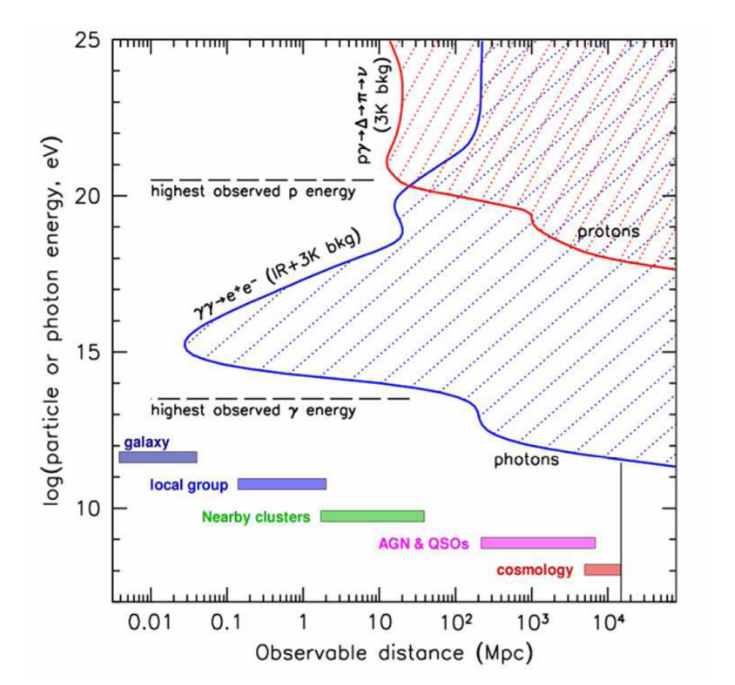
\includegraphics[width=0.8\textwidth]{figs/photevthorizon.png}
\caption{A plot of the photon and cosmic ray event horizons, showing the regions/energy scales visible using observations originating from photons (blue) and cosmic rays (red). Pair production of high energy photons with the ambient radiation in the universe prevents photon observations at long distances and high energies, including much of the energy scale below the highest observed cosmic ray energy. Also note that the photon event horizon can prevent us from studying the highest energy photons from AGN~\cite{Yuan_2011}. }
\label{fig:photeh}
\end{figure}

\section{Neutrinos}

\subsection{Production Mechanisms}
Neutrinos in astrophysical sources are produced via charged pion decay from pions produced from cosmic ray interactions with either photons or protons. The charge of the pion determines whether more neutrinos or anti-neutrinos are produced (eq. \ref{nuprodeq1} and \ref{nuprodeq2}):

\begin{equation}
    \pi^+ \rightarrow \nu_{\mu} + \mu^+ \rightarrow \nu_{\mu} + e^+ + \nu_{e}+\bar{\nu_{\mu}}
\label{nuprodeq1}
\end{equation}

\begin{equation}
    \pi^- \rightarrow \nu_{\mu} + \mu^- \rightarrow \bar{\nu_{\mu}} + e ^- + \bar{\nu_{e}}+\nu_{\mu}
\label{nuprodeq2}
\end{equation}

In either case, note that the expected flavor ratio of the neutrinos and anti-neutrinos produced at the source is $\nu_e : \nu_{\mu} : \nu_{\tau} = 1 : 2 : 0$. Combining this initial flavor ratio with neutrino oscillations over cosmic distances produces an expected observed astrophysical neutrino flavor ratio of $\nu_e : \nu_{\mu} : \nu_{\tau} = 1 : 1 : 1$.

Neutrinos are also produced by cosmic rays interacting with the Earth's atmosphere. This is referred to as the atmospheric neutrino flux, and has contributions both from pion decay ($\pi^+ \rightarrow \nu_{\mu} + \mu^+$, $\pi^- \rightarrow \bar{\nu_{\mu}} + \mu^-$), as well as kaon decay ($K^0_L \rightarrow \pi^\pm+ e^\mp +\nu_e$, $K^0_L \rightarrow \pi^\pm+ \mu^\mp +\nu_\mu$, $K^+ \rightarrow \mu^+ +\nu_\mu$, $K^+ \rightarrow \pi^0 + e^+ +\nu_e$, $K^+ \rightarrow \pi^0 + \mu^+ +\nu_\mu$). Below 100 TeV, the resultant spectrum closely follows that of cosmic rays, with a spectral index of $\gamma_{atmos}=2.7$. At higher energies the shower mesons are able to travel further in the atmosphere, giving them an increased opportunity to interact and steepening the spectral index to $\gamma_{atmos}=3.7$. The atmospheric neutrino flux exists as an irreducible background for many studies of the origin of astrophysical neutrinos. 

\subsection{Observed Neutrino Spectrum}
Both the astrophysical and atmospheric neutrino fluxes have been observed in data from the IceCube detector, with the astorphysical neutrino spectral index being measured to be $\gamma_{astro} \approx 2.28$ \cite{stettner2019measurement}.  While astrophysical and atmospheric neutrinos are largely indistinguishable on an individual event basis, the difference in spectra between the two populations ($\gamma_{astro} \approx 2.28$, $\gamma_{atmos} \approx 3.7$) allows us to distinguish between the two on a statistical basis. Higher energy events are more likely to be astrophysical in origin, and an equal share of astrophysical and atmospheric neutrinos can be expected at $\approx$ 200 TeV. Currently, the source(s) of the astrophysical neutrino flux have yet to be identified. For this reason, the observed astrophysical neutrino flux is commonly referred to as the "diffuse" astrophysical neutrino flux (as opposed to a "point source" flux, where specific astrophysical objects that are producing neutrino are identified).

\begin{figure}[h]
\centering
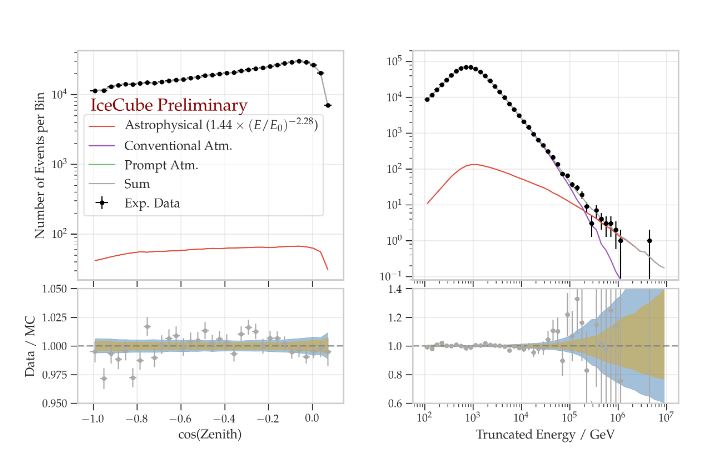
\includegraphics[width=0.8\textwidth]{figs/northerntracks_diffusefit.png}
\caption{Observation of the astrophysical neutrino flux in through-going tracks detected by the IceCube Neutrino Observatory. The effect is most visible in the plot of the observed energy spectrum on the right, showing the atmospheric contribution (blue) and the astrophysical contribution (red). The excess of events at high energies is unable to be explained without including a non-zero astrophysical contribution~\cite{stettner2019measurement}. }
\label{fig:diffusefit}
\end{figure}

\subsection{Neutrinos as Astrophysical Messengers}
As noted in the previous section, hadronic processes in astrophysical sources can produce neutrinos via pion decay. Like gamma rays, neutrinos are electrically neutral, and thus their paths are not bent by magnetic fields. Unlike gamma rays, however, neutrinos do not interact electromagnetically, instead interacting only via the weak force. Because of this, the mean free path of neutrinos traveling through the universe is significantly greater than that of photons, allowing us to use neutrinos to probe regions normally opaque to gamma rays. 

Astrophysical neutrinos are not without their drawbacks, however. The fact that neutrinos interact only weakly necessitates the construction of large detectors in order to observe an appreciable number of astrophysical events. Such detectors also observe a large, irreducible background of atmospheric neutrinos, particularly at lower (TeV) energies. For this reason, multi-messenger approaches that combine information from neutrinos and other astrophysical messengers are commonly used to attempt to identify the sources of astrophysical neutrinos. 


\subsection{AGN as Neutrino Source Candidates}
Since neutrinos can be used as an indicator of hadronic processes in astrophysical sources, identifying the source of the astrophysical neutrino flux is a promising route to also identifying the source of ultra-high energy cosmic rays. Though the source of the astrophysical neutrino flux has yet to be fully determined, in recent years there have been promising hints that extragalactic AGN are at least partially responsible.

An active galactic nucleus (AGN) is a compact region at the center of a galaxy displaying elevated electromagnetic emission, such that the additional luminosity cannot be attributed to stars. The luminosity is expected to originate from the accretion disk surrounding a supermassive black hole at the center of the galaxy, where conditions are thought to be ideal for high-energy particle acceleration and production.

The angle at which the AGN is viewed relative to its jet determines its exact classification, as can be seen in figure \ref{fig:AGNfig}. If the AGN is viewed "down" the jet (i.e. the jet is directed at Earth), the AGN is seen to be particularly luminous and is referred to as a blazar. Blazars can be further divided into two subclasses: flat spectrum radio quasars (FSRQ), which have luminous broad emission lines and continuous thermal emission, and BL-Lacs, which have weak or absent broad emission lines. AGN viewed off-axis fall into a variety of other classifications, with further sub-classification being defined by the spectrum of the AGN in various wavelength bands.

\begin{figure}[h]
\centering
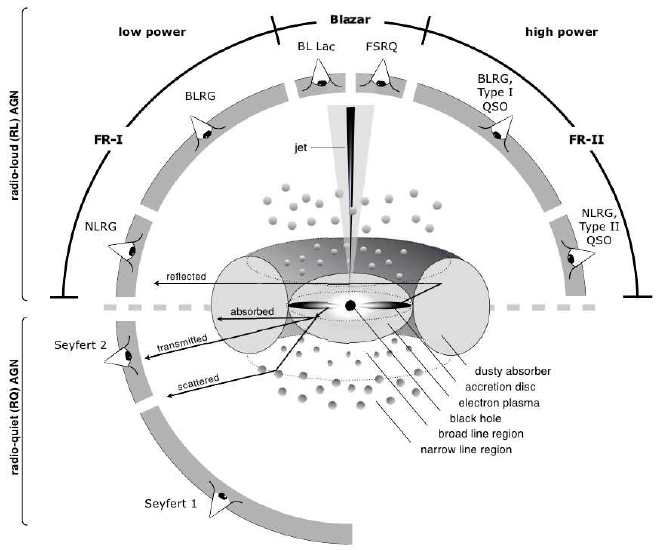
\includegraphics[width=0.8\textwidth]{figs/AGNfig.png}
\caption{The unified AGN model, showing the various classifications of AGN for different observation angles. If the jet is directed at Earth, the object is viewed as a blazar, while other viewing angles can obscure the jet, leading to alternative classification (e.g. as a Seyfert galaxy)~\cite{AGN_model_src}. }
\label{fig:AGNfig}
\end{figure}

\subsubsection{TXS 0506+056}
On September 22, 2017, the IceCube Neutrino Observatory detected a high energy neutrino, IceCube-170922A, with an energy of approximately 290 TeV. The arrival direction of IceCube-170922A was consistent with the location of the blazar TXS 0506+056, and sparked multi-messenger followup from a variety of other telescopes and detectors. Notably, it was determined that TXS 0506+056 was flaring in gamma rays at the time IC-170922A was observed. The significance of the positional correlation of a high energy IceCube event and a flaring blazar was calculated to be $3.0 \sigma$, providing the first hint that blazars may be a source of high energy astrophysical neutrinos~\cite{TXS_Multimessenger}.

\begin{figure}[h]
\centering
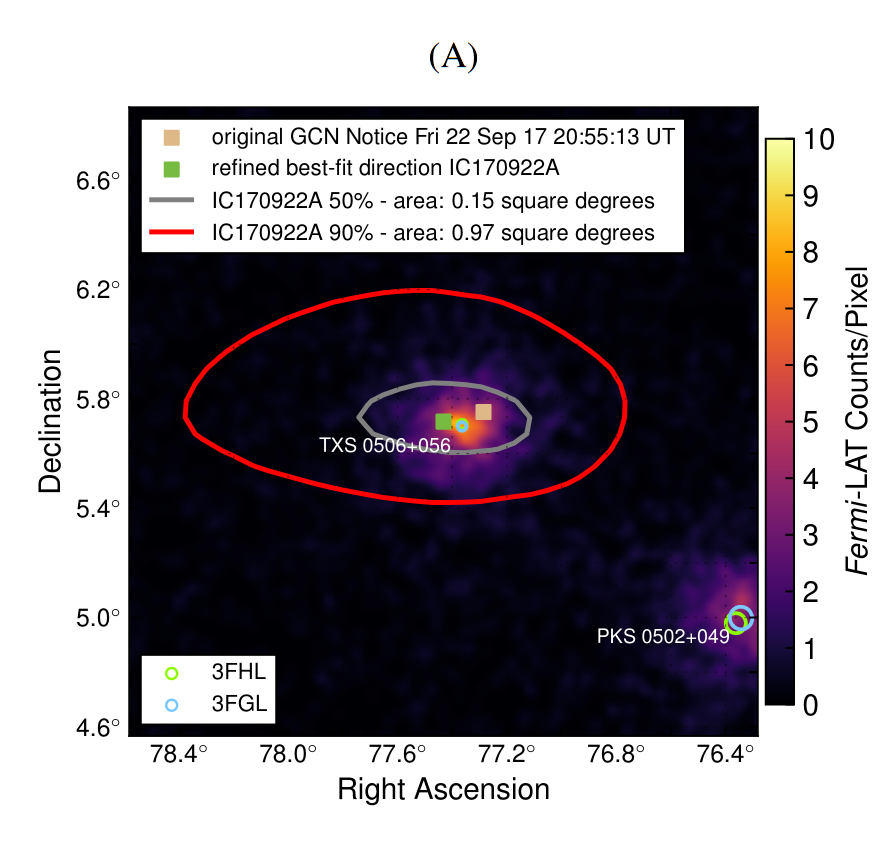
\includegraphics[width=0.8\textwidth]{figs/FermiMap.png}
\caption{The Fermi-LAT skymap near the location of the observed high energy IceCube event IC170922A, with the 50\% and 90\% error contours associated with IC170922A plotted in grey and red, respectively. The significance associated with the spatial coincidence of the high energy event and TXS 0506+056 was found to be $3.0 \sigma$~\cite{TXS_Multimessenger}. }
\label{fig:FermiMap}
\end{figure}

In addition to examining the multi-messenger correlation of a high energy IceCube event and a flaring blazar, an analysis of archival IceCube data was performed at the coordinates of IC170922A, examining the historical behavior of neutrino emission from this location of the sky over the previous nine years. In addition to the original high energy event observed in 2017, this archival analysis also revealed a 158 day period of elevated neutrino emission beginning in September 2014. The significance of this archival "neutrino flare" was calculated to be $3.5\sigma$. Unlike the 2017 high energy event, the 2014 neutrino flare did not correspond to a flaring period for TXS 0506+056 in gamma rays.~\cite{TXS_Archival}

\begin{figure}[h]
\centering
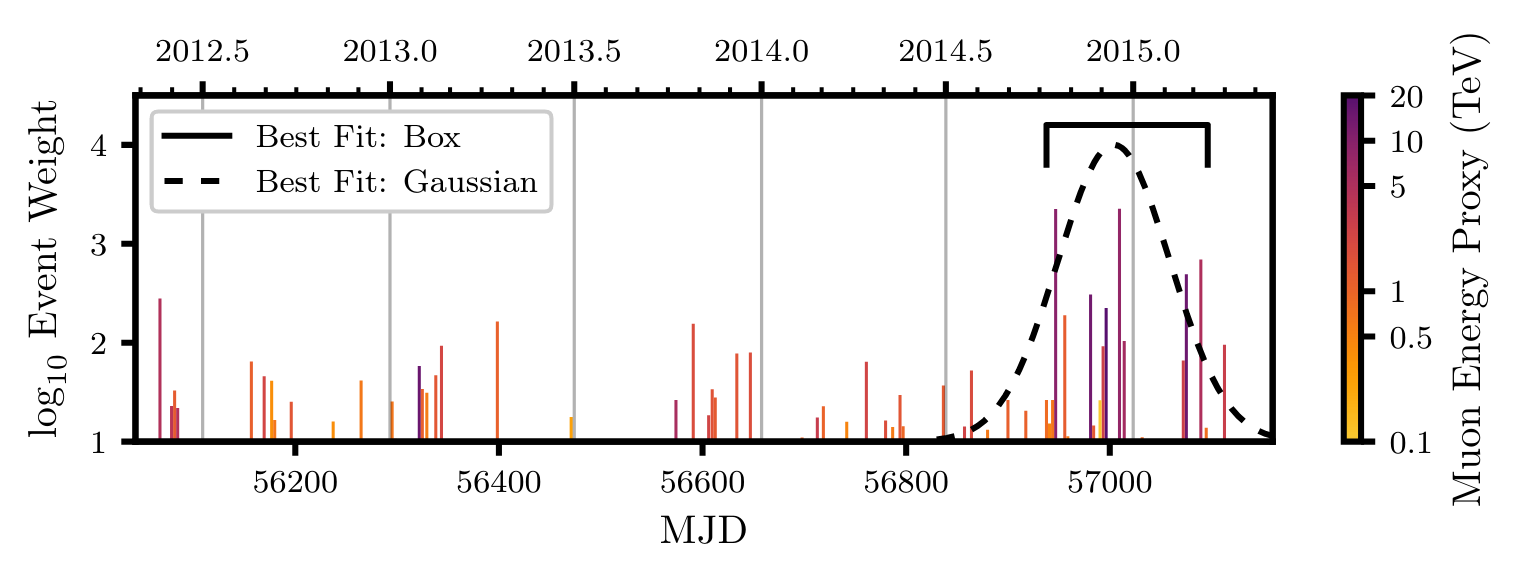
\includegraphics[width=0.8\textwidth]{figs/TXS_flarecurve.png}
\caption{The result of the archival analysis of IceCube data near the location of TXS 0506+056, with the $3.5\sigma$ flare shown. This flare is separate from the high energy event observed in 2017, and there was no corresponding flare observed in gamma rays during this time period~\cite{TXS_Archival}. }
\label{fig:TXS_flarecurve}
\end{figure}

The combination of a $3.0 \sigma$ multimessenger result with the $3.5 \sigma$ "untriggered" neutrino flare in 2014 suggest a significance of TXS 0506+056 as a neutrino source of at least $3 \sigma$. This makes for a strong argument for extragalactic blazars as interesting source candidates from the perspective of neutrino astronomy. 

\subsubsection{NGC 1068}
In addition to the multimessenger and archival results associated with TXS 0506+056, the results of the 10-year time integrated IceCube analysis~\cite{10yr_tint} also seem to suggest AGN as candidates for astrophysical neutrino emission. In this all-sky, untriggered, time integrated analysis, the most significant point in the northern sky appears to be spatially coincident with the Seyfert II galaxy NGC 1068. Notably, NGC 1068 was also included in an associated time integrated catalog analysis. In this catalog analysis, the pre-trial significance of time-integrated neutrino emission from NGC 1068 was $1.8 \times 10^{-5}$, corresponding to a significance of $2.9\sigma$. At a 14.4 Mpc distance, NGC 1068 is the most luminous Seyfert II galaxy detected by Fermi-LAT, and NGC 1068 had additionally been hypothesized as a candidate cosmic ray accelerator prior to this particular analysis\ \cite{NCG_1}\cite{NGC_2}\cite{NGC_3}.

It should additionally be noted that the catalog analysis mentioned above identified three other objects which, together with NGC 1068, collectively form a $3.3\sigma$ excess over the background expectation. These objects are the Seyfert II galaxy NGC 1068, the blazar TXS 0506+056,and the BL Lacs PKS 1424+240 and GB6 J1542+6129 \cite{10yr_tint}, providing further indication of AGN as potential neutrino emitters. 

\begin{figure}[h]
\centering
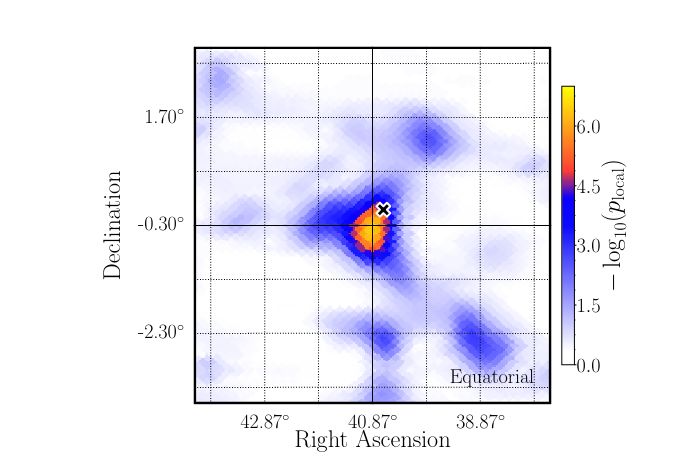
\includegraphics[width=0.8\textwidth]{figs/NGC_tint.png}
\caption{The results of the untriggered time integrated IceCube point source search analysis, showing the most significant spot in the northern sky, with the location of NGC 1068 plotted as the black "X"~\cite{10yr_tint}. }
\label{fig:NGC_tint}
\end{figure}


\subsection{Galactic Neutrino Sources}
Though this work will primarily focus on searches for extra-galactic point sources of the astrophysical neutrino flux, potential neutrino emission from sources within our galaxy is an active area of study as well. Notably, one of the first confirmed sources of lower energy astrophysical neutrinos was Supernova 1987A \cite{Bionta:1987qt}, a supernova occurring within the Milky Way. Other galactic objects that are considered candidates for neutrino emission include supernova remnants \cite{snr_2020}, as well as pulsar wind nebula \cite{pwn_2020}, both of which are known to produce gamma rays. 

The majority of the galactic plane lies in the southern sky. Since neutrino telescopes make use of the earth to block out atmospheric muon backgrounds (see subsequent chapter), this means that to best study the galactic plane, a neutrino observatory located in the northern hemisphere would be required. While there are several such telescopes either planned or under construction \cite{Agostini_2020}\cite{kappes2007km3net}, they have yet to reach effective volumes comparable to the existing IceCube observatory (located in the southern hemisphere). 

\subsection{Constraints on Neutrino Source Populations from Diffuse Measurements}
It is important to keep in mind that whatever the sources of astrophysical neutrinos may be, they must combine to reproduce the measured diffuse astrophysical neutrino flux. The current best fit astrophysical neutrino spectrum, assuming a single power law in energy, is given as (eq. \ref{diffuse_fit})~\cite{stettner2019measurement}:

\begin{equation}
    \frac{d\phi_{\nu+\bar{\nu}}}{dE} = 1.44_{-0.24}^{+0.25} (\frac{E}{100 \textrm{TeV}})^{-2.28_{-0.09}^{+0.08}} 10^{-18} \textrm{GeV}^{-1}\textrm{cm}^{-1}\textrm{s}^{-1}\textrm{sr}^{-1}
\label{diffuse_fit}
\end{equation}

This places constraints on the density and luminosity of potential astrophysical neutrino source populations. If a candidate source population has sources that are too numerous and/or too bright, then that source population would produce a higher flux of astrophysical neutrinos than has been observed, and an explanation of the nondetection of the additional flux is required. Similarly, if sources are too sparse and/or too dim, then such a source class is incapable of explaining the entirety of the measured diffuse flux. 

These constraints can be summarized in figure \ref{fig:muraseplot}, showing the band of the measured diffuse flux in source density/luminosity space, as well as several commonly discussed source populations. It should be noted that in this plot, the luminosity values for various source populations are derived from the electromagnetic luminosity $L_\gamma$. In principle, the true ratio $L_\nu/L_\gamma$ remains unknown, and consequently the positions of sources along the luminosity axis may shift according to this value. 


\begin{figure}[h]
\centering
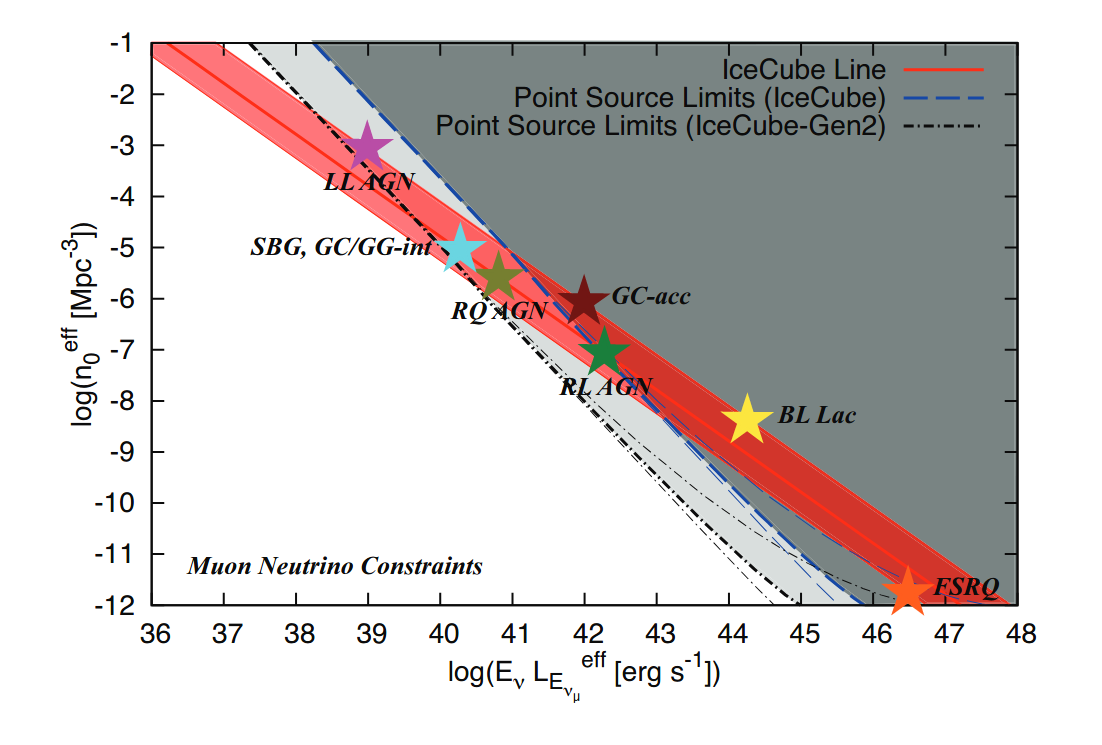
\includegraphics[width=0.8\textwidth]{figs/muraseplot.png}
\caption{Constraints on potential populations of sources of the high energy astrophysical neutrino flux. The red band represents combinations of source density and luminosity that are consistent with the measured astrophysical neutrino flux. Source populations that lie above this band are too bright and/or too numerous, while source below this band are too dim/too sparse. Also shown are limits derived from the non-observation of neutrino sources in time-integrated analyses performed by the IceCube collaboration as of 2016, as well as a projected set of limits that would be associated with a non-observation from IceCube-Gen2~\cite{Murase_constraints}. }
\label{fig:muraseplot}
\end{figure}

